% Dossier de qualité
% Version 16.64

% Historique des versions
% fichtre!! on y fera sur les prochains dossier.

\documentclass[a4paper, 11pt]{article}

\usepackage[utf8]{inputenc} % Texte en utf-8
\usepackage{aeguill} % Coupure des mots accentués
\usepackage[francais]{babel} % Typographie française
\usepackage[pdftex, hypertexnames=false, colorlinks=true, final]{hyperref}
\usepackage[final]{graphicx}
\usepackage{url} % Gestion des URLs
\usepackage{geometry}
\usepackage{fancyhdr}

\DeclareGraphicsRule{.svg}{png}{.png}{`convert #1 `basename #1 .svg`.png}

% Marges à gauche et à droite de 3cm
\geometry{margin=3cm}

% Utilisation des headers et footers personnalisés de fancyhdr
\pagestyle{fancy}

% Images dans le dossier ./images/
\graphicspath{{./images/}}

% Gestion des métadonnées étranges à rendre visibles au rendu
\newcommand\docname{STBv1.1}
\newcommand\docauthor{Pierre-Yves David --- Rémi Thévenoux}
\newcommand\docstatus{LIVRABLE} % EN COURS, ATTENTE, VALIDE ou LIVRABLE

% Numérotation mieux
%\renewcommand\thechapter{\Alph{chapter}}
%\renewcommand\thesection{\Roman{section}}
%\renewcommand\thesubsection{\arabic{subsection}}
%\renewcommand\thesubsubsection{\alph{subsubsection}}

% Format de citation de références standard, marche avec quasiment tout
\newcommand\fullref[1]{\ref{#1}, page \pageref{#1}}

% En-têtes et pieds de page
\lhead{\docname}
\rhead{}
\lfoot{Auteur : H4213}
\cfoot{}
\rfoot{\thepage}

% Titre du document maître
\title{\textbf{COPEVUE}\\
\rule{\textwidth}{1pt}{}\\
\Huge{\textsc{Spécification Technique des Besoins}}}
\author{\docauthor{} (H4213)}
\date{\docname{} --- \today{} (\docstatus{})}

\begin{document}

\maketitle

\tableofcontents

\pagebreak

% STB + Annexes : 10 pages maxi

\section{Axes d'amélioration}
\subsection{Axes de progrès retenus}
\subsubsection{Améliorer la disponibilité des sites isolés}
S'assurer que les sites isolés maintiennent toujours leurs capacités opérationnelles~-- réservoir plein, personne âgée en vie, etc.
\subsubsection{Améliorer la maintenance}
Détecter au plus tôt les anomalies et identifier les pannes potentielles. Agir automatiquement sur les sites isolés en cas de problème ou avertir un système central.
\subsubsection{Améliorer la logistique}
\begin{itemize}
\item Prévoir à l'avance les interventions nécessaires et optimiser le trajet des intervenants.
\item Pouvoir mettre à jour les trajets en fonction des interventions imprévues~-- fuite d'un réservoir, détresse cardiaque, etc.
\item Améliorer la logistique implique une réduction des coûts et une amélioration de la réactivité.
\end{itemize}

\subsection{Axes de progrès marginaux}
\subsubsection{Mettre en place un suivi et un archivage}
Stocker l'ensemble des données~-- mesures et interventions~-- de manière fiable et sécurisée durant la durée légale minimale. Possibilité de suivre les évolutions des données.
%\subsubsection{Diminution des risques environementaux}

\section{Architecture générale de la solution}
Pour définir les spécifications, nous avons découpé la solution générale en six sous-systèmes ayant chacun ces spécifications :

\begin{figure}[!htp]
\begin{center}
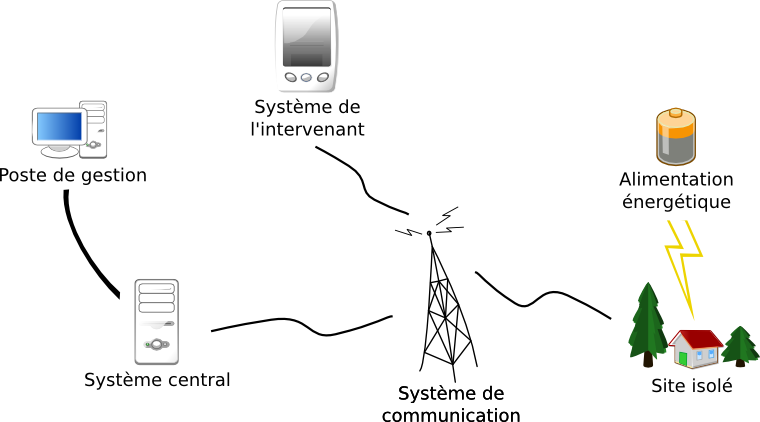
\includegraphics[width=.7\textwidth]{schema_architecture_generale.png}
\caption{Architecture générale}
\label{figure:schema_architecture_generale}
\end{center}
\end{figure}

\begin{description}
	\item[Le site isolé] qui correspond à l'ensemble du matériel et de l'applicatif des sites isolés en dehors de l'alimentation énergétique.
	\item[L'alimentation énergétique] est le système permettant de fournir l'énergie aux sites isolés.
	\item[Le système central] est le système où sont stockées toutes les données et où sont effectués les traitements de celles-ci.
	\item[Le poste de gestion] est le poste permettant de configurer le système central ainsi que de visualiser des données.
	\item[Le système de l'intervenant] est le système permettant à l'intervenant de recevoir et d'envoyer des informations pendant ces interventions.
	\item[Le système de communication] est le système permettant la communication entre le système central, les sites isolés et le système de l'intervenant.
\end{description}

\section{Description des exigences fonctionnelles}
\subsection{Système central}
Le système central doit permettre de :
\begin{description}
	\item [Stocker les données reçues] pour permettre leur traitement.
	\item [Archiver des données] pour permettre le suivi et la relecture ultérieure si nécessaire, on veillera à une taille d'archivage suffisante.
	\item [Prévoir les interventions] aussi bien pour permettre le maintien de la fonctionnalité du site~-- remplir une cuve d'essence, etc.~-- que les interventions de maintenance préventive.
	\item [Calculer l'itinéraire des intervenants] à partir des prévisions d'intervention et des dernières informations reçues.  
\end{description}

\subsection{Poste de gestion}
Le poste de gestion doit permettre de :
\begin{description}
	\item [Se connecter au serveur central] pour pouvoir le configurer et en extraire des données.
	\item [Paramétrer le serveur central] pour modifier les configurations de stockage et de traitement des données ou le calcul d'itinéraires.
	\item [Extraire des données du central] afin de pouvoir visualiser le suivi des mesures et interventions.
	\item [Gérer la configuration des sites isolés] pour régler le fonctionnement de la chaîne de mesure, des alertes, de la communication, etc.
	\item [Effectuer des actions sur les sites isolés] afin de faire de la maintenance préventive ou curative, ou toute autre opération utile.
\end{description}

\subsection{Système de l'intervenant}
Le système de l'intervenant doit permettre de :
\begin{description}
	\item [Se connecter au système de communication] pour recevoir les informations, notamment l'itinéraire.
	\item [Recevoir l'itinéraire] de la tournée d'intervention.
	\item [Géolocaliser l'intervenant] afin de faciliter sa conduite et trouver facilement les sites isolés.
	\item [Permettre une connexion locale avec le site isolé] afin de permettre une communication en cas de dysfonctionnement du système de communication.
	\item [Configurer et extraire des données du site isolé] afin de pouvoir faire de la maintenance sur site.
\end{description}

\subsection{Système de communication}
Le système de communication doit être capable de :
\begin{description}
	\item[Établir des connexions point à point] entre le système central, les sites isolés et le système des intervenants.
	% version PY : entre le serveur et le client.
\end{description}

\subsection{Site isolé}
Le site isolé doit être capable de :
\begin{description}
	\item[Lire un capteur] pour transmettre ou vérifier sa valeur.
	\item[Se réveiller régulièrement] pour lire les valeurs de ses capteurs et les envoyer au serveur central à intervalles réguliers\footnote{Les communications avec le serveur étant relativement coûteuses, les valeurs pourront être lues plus souvent qu'elles ne sont transmises}.
	\item[Détecter une erreur] en vérifiant les valeurs lues par les capteurs et leurs variations. Une fois l'erreur détectée, le site doit prendre la mesure possible localement et prévenir le serveur central.
	\item[Offrir une connexion extérieure] pour permettre aux agents humains de relever des valeurs ou enclencher des actions directement.
	\item[Permettre une connexion au système de communication global] afin de relier le site isolé et le système central directement.
	\item[Permettre une connexion physique locale] afin d'assurer la connexion en cas de défaillance du système principal.
	\item[Se géolocaliser] afin de communiquer sa position aux intervenants et au système central. La géolocalisation ne sera nécessaire que si le site isolé est mobile.
\end{description}

\subsection{Alimentation énergétique}
L'alimentation énergétique doit permettre de :
\begin{description}
\item[Alimenter en électricité] le site isolé.
\end{description}



\section{Description des exigences non fonctionnelles du futur système}
\subsection{Système central}
	\subsubsection{Pérennité}
	 Le système d'archivage doit être complètement sécurisé et garantir la sauvegarde des informations tout au long de la période de stockage.
	\subsubsection{Fiabilité}
	Le système doit être complètement fiable autant au niveau du matériel qu'au niveau logiciel.
	\subsubsection{Interopérabilité}
	La sauvegarde des données doit se faire dans un format permettant l'interopérabilité afin de permettre des évolutions du système de sauvegarde ainsi que la lecture depuis des applications extérieures chargées d'analyser les données.
	\subsubsection{Puissance}
	Le système n'a pas besoin d'une grande rapidité mais la puissance de calcul doit être suffisante pour pouvoir traiter une grande quantité de données.
	
\subsection{Poste de gestion}
	\subsubsection{Simplicité}
	Toutes les fonctions permises devront être facilement utilisables par l'opérateur qui ne sera pas forcément une personne familière avec l'informatique.
	\subsubsection{Compatibilité}
	Le poste doit pouvoir se connecter facilement avec le système central afin d'en extraire des données et de le paramétrer.
		
\subsection{Système de l'intervenant}
	\subsubsection{Simplicité}
	Toutes les fonctions permises devront être facilement utilisables par l'opérateur qui ne sera pas forcément une personne familière avec l'informatique.
	\subsubsection{Rapidité de programmation}
	Le système de l'intervenant doit permettre une programmation rapide et efficace.
	\subsubsection{Compatibilité}
	Le poste doit pouvoir se connecter facilement avec le site isolé afin d'en extraire des données et de le paramétrer.

\subsection{Système de communication}
	\subsubsection{Disponibilité}
		Tous les sites isolés doivent pouvoir avoir accès au système de communication.
	\subsubsection{Fiabilité du transfert}
		Les différents clients du système doivent pouvoir s'assurer du transfert correct des données.
	\subsubsection{Autonomie}
		La maintenance du système ne doit pas être excessivement alourdie par le déploiement du réseau.
	\subsubsection{Robustesse}
		Le système de communication doit être opérationnel malgré des conditions climatiques défavorables.

\subsection{Site isolé}
	Tout l'appareillage déployé sur le site isolé doit disposer d'un certain nombre de qualités pour garantir la viabilité de la solution.
	\subsubsection{Robustesse au milieu}
	Les milieux où sont déployés de tels appareils peuvent avoir des caractéristiques extrêmes auquelles le système doit pouvoir résister. Dans le cas de la Norvège, celles-ci sont :
    \begin{itemize}
		\item le gel,
		\item la neige,
		\item les perturbations électromagnétiques,
		\item les animaux sauvages.
	\end{itemize}
	\subsubsection{Autonomie}
		Les besoins en énergie et la plupart des pannes doivent pouvoir se résoudre eux-mêmes automatiquement sans nécessiter une intervention humaine. En particulier, si le fonctionnement du système est bloqué par des conditions extérieures, le système doit pouvoir se réarmer seul lorsque les conditions permettent de nouveau un fonctionnement normal.
	\subsubsection{Économie d'énergie}
		Tous les composants du système doivent avoir une consommation d'énergie minimum pour limiter les besoins d'énergie et améliorer l'autonomie.
	\subsubsection{Fiabilité}
		Les composants du matériel et de l'applicatif seront sélectionnés parmi des composants ayant démontré leur fiabilité.
	\subsubsection{Fiabilité et précision des mesures}
		La précision des mesures doit correspondre aux besoins propres de la fonctionnalité du site. La fiabilité sur ces mesures doit être irréprochable.
	\subsubsection{Flexibilité du positionnement}
		Le site isolé doit pouvoir déployer les capteurs et actionneurs sur un rayon pouvant aller jusqu'à une centaine de mètres.
	\subsubsection{Miniaturisation}
		Les besoins en miniaturisation dépendront du type de site isolé. Pour le cas de la Norvège, nous préférerons assurer l'autonomie énergétique au détriment de la miniaturisation. En revanche, pour le cas des personnes âgées, la miniaturisation sera un besoin important.
	\subsubsection{Logiciels adaptés}
		\begin{itemize}
			\item OS : petite taille en mémoire.
			\item OS : support de la veille.
			\item connexion locale : facile à implémenter.
	\end{itemize}
	
\subsection{Alimentation énergétique}
	\subsubsection{Autonome}
	L'alimentation doit nécessiter le moins possible d'interventions sur site, avec quelques accès par an pour les sites plus compliqués d'accès.
	Entre deux interventions, l'alimentation doit être suffisante pour \emph{la pire consommation possible}, notamment l'activation de toutes les procédures d'urgence.
	\subsubsection{Maintenabilité}
	La maintenabilité de l'alimentation devra être la plus simple possible pour simplifer au maximum les opérations lors des interventions.
	\subsubsection{Robuste}
    L'alimentation doit être efficace malgré des conditions climatiques défavorables, notamment par grand froid.

\section{Impacts de la nouvelle solution sur le système}
\subsection{Axes principaux}
\subsubsection{Améliorer la maintenance}
Les mesures sur sites permettent de détecter des anomalies et d'intervenir sur le site s'il possède les actionneurs nécessaires ou bien d'alerter le système central si une intervention est nécessaire. Cela permet d'intervenir dès les premiers signes d'une anomalie et d'éviter des conséquences lourdes, ainsi que d'automatiser la maintenance.
\subsubsection{Améliorer la disponibilité des sites isolés}
Le suivi des sites isolés permet d'anticiper les interventions et donc d'agir avant que le site ne soit plus opérationnel. L'amélioration de la maintenance permet aussi d'améliorer la disponibilité en minimisant les temps de carence.
\subsubsection{Améliorer la logistique}
La récolte des données et leur suivi permet d'anticiper les besoins d'intervention sur les sites isolés. Grâce à ce système, nous pouvons planifier l'itinéraire des intervenants et optimiser celui-ci. De plus, la possibilité de communiquer avec les intervenants permet de modifier leur itinéraire si besoin est.
\subsection{Axes secondaires}
\subsubsection{Mettre en place un suivi et un archivage}
Le stockage des données sur le serveur central permet un archivage efficace sur le long terme et la possibilité de mettre en place des outils de suivi.

\section{Bilan des améliorations}
La majorité des améliorations que nous prévoyons de mettre en place concerne l'optimisation de la surveillance des sites isolés. Elle concerne autant la fiabilité de système que la planification des tâches, le but étant d'assurer un fonctionnement en continu de chacun des sites. Ces contraintes sont fonctionnelles, c'est la raison d'être du système déployé. Il est nécessaire que chaque site soit fonctionnel le plus souvent possible, l'optimum visé étant une disponibilité permanente. Si ceux-ci tombent en panne, le nécessaire doit être fait pour permettre une remise en service rapide : reprise automatique, intervention humaine, etc. Les phases préliminaires~-- conception~-- et d'exploitation~-- planification, maintenance~-- prennent en compte ces critères et intègrent une notion d'optimisation.  

Dans un second temps, nous traitons les contraintes non fonctionnelles telles que l'amélioration de la logistique ou la mise en place d'un archivage. Ces améliorations très importantes pour le bon fonctionnement du système ne sont cependant pas critiques, même si une bonne gestion logistique influencera positivement l'état de fonctionnalité de chaque site.

%%%%%%%%%%%%%%%%%%%%%%%%%%%%%%%%%%%
%%%%%%%% Fin du dossier %%%%%%%%%%%
%%%%%%%%%%%%%%%%%%%%%%%%%%%%%%%%%%%

\end{document}